\documentclass{article}
\setlength{\headheight}{33pt}

\usepackage[
  top=1.8cm,
  bottom=1.5cm,
  left=1.8cm,
  right=1.8cm,
  includefoot,
  includehead]{geometry}

\usepackage[utf8]{inputenc}
\usepackage{changepage}
\usepackage{multicol}
\usepackage{nccmath}
\usepackage{amsmath}
\usepackage{graphicx}
\usepackage{calc}
\usepackage{enumitem}

% For fancy math
\RequirePackage{amsmath,amsthm,amssymb}
\newtheorem{theorem}{Theorem}
\newtheorem{fact}[theorem]{Fact}
\newtheorem{lemma}[theorem]{Lemma}
\newtheorem{claim}[theorem]{Claim}

\newcommand{\ord}[2][th]{\ensuremath{{#2}^{\mathrm{#1}}}}
% shorthand for \mathcal{O}
\newcommand{\Ocal}{\ensuremath{\mathcal{O}}}
\newcommand{\aug}{\fboxsep=-\fboxrule\!\!\!\fbox{\strut}\!\!\!}
\newcommand{\contradiction}{%
  \ensuremath{{\Rightarrow\mspace{-2mu}\Leftarrow}}%
}

\graphicspath{{./images}}

% Counters for HW number, author, and collaborators
\newcommand{\hwnumber}[1]{\def\hwnumberdata{#1}}
\def\hwnumberdata{\relax}
\renewcommand{\author}[1]{\def\authordata{#1}}
\def\authordata{\relax}
\newcommand{\collaborators}[1]{\def\collaboratorsdata{#1}}
\def\collaboratorsdata{\relax}

% Fancy headings
\RequirePackage{fancyhdr}
\pagestyle{fancyplain}

\fancyhead[L]{\small \authordata \\
\small CS 630 Homework \#\hwnumberdata \\
  \textsl{Collaborators}: \collaboratorsdata}

\RequirePackage{titlesec}
\titleformat{\subsection}{\normalsize\bfseries}{\thesubsection}{.5em}{}
\renewcommand{\thesubsection}{\alph{subsection})}

% Making the problem and ppart environments
\newcommand{\addmedskip}{\addvspace{2\medskipamount}}
\newcommand{\addbigskip}{\addvspace{2\bigskipamount}}
\newcommand{\nline}{\bigskip}

\newcounter{problemnum}
\setcounter{problemnum}{0}
\newenvironment{problem}
  {\addbigskip \setcounter{partnum}{0}
   \noindent\stepcounter{problemnum}\textbf{Problem \arabic{problemnum}.\ }}
  {\par\addbigskip}

\newcounter{partnum}
\setcounter{partnum}{0}

\newenvironment{ppart}[1][]{%
  \addmedskip
  \refstepcounter{partnum}%\par\medskip%
  \enumerate[labelsep=*]\item[\textbf{\roman{partnum})}]}
  {\endenumerate}

\newsavebox{\mybox}
\newenvironment{answer}
{\begin{lrbox}{\mybox}\begin{minipage}{0.95\textwidth}\vspace{0.2cm}}
  {\vspace{0.1cm}\end{minipage}\end{lrbox}\fbox{\usebox{\mybox}}}

\newenvironment{customProof}{\begin{proof}\noindent}{\end{proof}}

% Put your name and the homework number here.
\author{Jiun-Yan (Eric) Chen}
\hwnumber{4}


\begin{document}
\vspace*{0.5\baselineskip}
\textbf{Please limit your answer to the following problems to at most 1/2 a page each.}

\collaborators{None} % Put your collaborators for the problem here
\begin{problem}

    \nline
    
    \begin{answer}
        We can reduce the Boolean Satisfiability Problem into a Clique Problem.

        For each variable in SAT in the conjunctive normal form, we create a vertex representing this this variable, along with a secondary value denoting the group number. (Use the order of the group in SAT for simplicity).

        Connect each vertex in our graph to another vertex if:
    
        1. The other vertex has is not the opposite ($x_1$, $\neg x_1$ are opposites)
        2. The other vertex is in a different group.

        The original problem is satisfiable if there is a clique of size $m$, where $m$ is the number of groups in the equation, in this generated graph.

        Since we can perform this transformation in $n^2$ time, and we know that SAT is also NP. That means that the Clique Problem is also in NP.
    \end{answer}

\end{problem}

\newpage

\collaborators{None} % Put your collaborators the problem here
\begin{problem}

    The problem here is to give an example of a complete weighted but NON-Euclidean graph G with 4 or 5 vertices which has the property that when you run the 2-approximation for the traveling saleman problem on the graph, you obtain a TSP solution whose value is more than 20 times the optimal TSP solution for that graph.

    \begin{ppart}
        Draw your example weight graph G, and state whawt makes it non-Euclidean.
    \end{ppart}

    \begin{answer}
        \noindent\begin{minipage}{0.3\textwidth}% adapt widths of minipages to your needs
            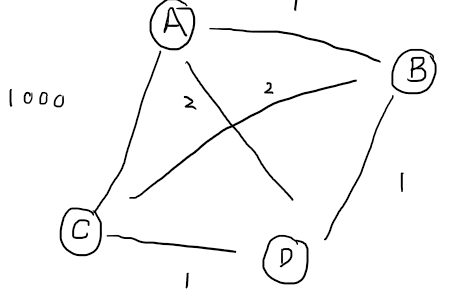
\includegraphics[scale=0.4]{2-1.png}
            \end{minipage}%
            \hfill%
            \begin{minipage}{0.6\textwidth}
                This is non-euclidean because the triangle formed by A, B, C have the edges 1, 2, 1000, which is an impossible euclidean triangle.
            \end{minipage}
    \end{answer}

    \begin{ppart}
        Show what the optimal solution for G is, and if possible explain your answer.
    \end{ppart}


    \begin{answer}
        The optimal solution is the path A-D-C-B-A, which gives a total path cost of 6.
    \end{answer}

    \begin{ppart}
        Give the result of running the 2-approximation algorithm and show the steps you went through to get this approximation.
    \end{ppart}

    \begin{answer}
        Start with node A.
        
        1. Next minimum cost node is B

        2. Next minimum cost node is D

        3. Next minimum cost node is C

        4. Add A back into the list.

        Total cost for A-B-D-C-A is 1003.
    \end{answer}

    \nline

    Give an example of a complete Euclidean graph on G with at least 4 vertices where the 2 approximation for the traveling salesman problem on the graph G yields a TSP solution whose value is more than 1.6 times the optimal TSP soluiton for that graph. Show enough of your work so that the validity of your example is clear.

    \begin{answer}
       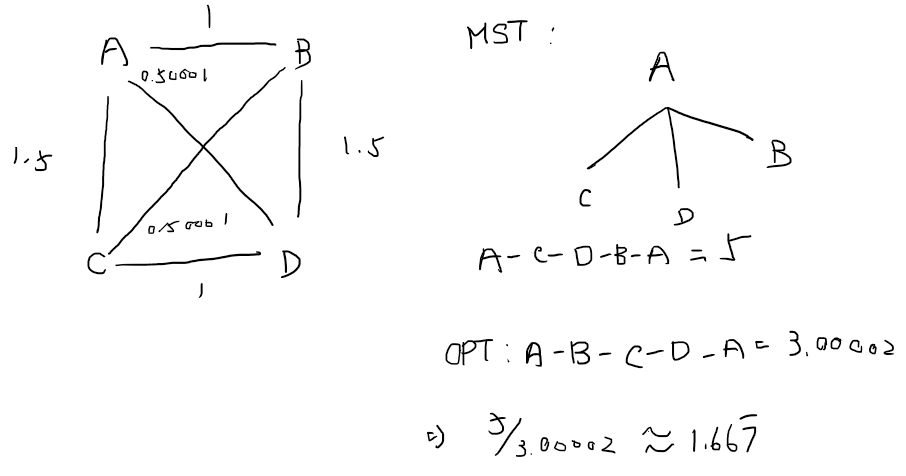
\includegraphics[scale=0.4]{2-2.png}
    \end{answer}
\end{problem}

\newpage

\begin{problem}
    Suppose that we are given a set of n objects, where the size $s_i$ of the $i$h object satisfies $0 < s_i < 1$. We wis hto pack all the objects into the minimum nnumber of unit-size bins. Each bin can hold any subset of the objects whose total size does not exceed 1.

    \begin{ppart}
        Prove that the problem of determining the minimum number of bins required is NP-hard.
    \end{ppart}

    \begin{answer}
        The bin-packing problem is an optimization problem that has the corresponding decision problem of whether the objects can be packed into some number of bins.

        We can generalize this into solving a subset sum problem where we are trying to find a subset of items that has sums closest to 1, and we repeat this problem n times for n bins.

        Since we know that the subset problem is NP-Hard, and the bin-packing problem is at least as hard as the subset problem, therefore, bin-packing problem is also NP-Hard
    \end{answer}

    \begin{ppart}
        Argue that the optimal number of bins required is at least $\lceil S \rceil$
    \end{ppart}

    \begin{answer}
        The amount of spaces need without regards to bin size limitations would be the sum size of each item, or S. Since each bin is a unit size, there must be at least $\lceil S \rceil $ bin to have a total size of S or more
    \end{answer}

    \begin{ppart}
        Argue that the first-fit heuristic leaves at most one bin less than half full.
    \end{ppart}

    \begin{answer}
        For a first-fit algorithm to place to create a new bin, there must not be an earlier bin that can fit this new item. If this new item $I$ creates a bin that is less than half full, and there was previously already a bin $B$ that was less than half full, then the sum of the item $I$ and the items in $B$ would be less than 1, and thus $I$ would not be placed into a new bin. Thus a second bin that is less than hal full would never be created if there was previously a bin that was also less than half full. Thus, the first-fit heuristic must always leave at most one bin less than half full.
    \end{answer}

    \begin{ppart}
        Prove that the number of bins used by the first-fit heuristic is never more than $\lceil 2S \rceil$
    \end{ppart}

    \begin{answer}
        From our previous problem we know that there must be at most 1 bin that is less than half full. This means that for a solution of K + 1 bins, there are K bins which are at least half full. Let the amount stored in the last bin be of size B. As these K bins will have a minimal stored item sum sie of 0.5K, we know that $0.5K + B < S$, which can be translated into $K < 2(S - B) => K < 2S$. Therefore, the number of bins used is never more than $\lceil 2S \rceil$
    \end{answer}

    \begin{ppart}
        Prove an approximation ratio of 2 for the first-fit heuristic
    \end{ppart}

    \begin{answer}
        From \textbf{ii} we know that the minimal amount of bins required is $\lceil S \rceil$, and from \textbf{iv} we know that the maximum amount of bins is less than $\lceil 2S \rceil$. 

        \nline

        Let $U = \lceil S \rceil - S, V = \lceil 2S \rceil - 2S$, $2 \lceil S \rceil = 2S + 2U$. If $U > 0.5$, then $V < 0.5 < 2U$. If $U < 0.5, V < 2U$. Therefore, $\lceil 2S \rceil = 2S + V < 2S + 2U = 2 \lceil S \rceil$, and the first-fit heuristic has an approximation ratio of 2.
    \end{answer}
\end{problem}

\newpage

\begin{problem}
    Recall the greedy set cover algorithm which was discussed in section and in our textbook. For this heuristic every step of the algorithm adds to the set cover the set i F which covers the most elements from U which are not yet covered by the algorithm.
    
    \begin{ppart}
        True or false: There is an instance I of the set cover problem on which the greedy set cover algorithm produces an answer which is $\ge OPT(I) + 2$. Explain your answer
    \end{ppart}
    
    \begin{answer}
        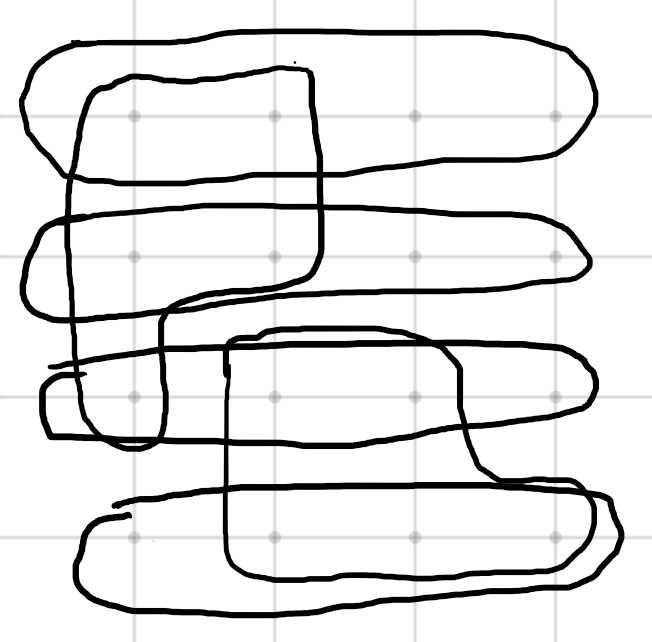
\includegraphics[scale = 0.5]{4-1.png}
        
        In the above instance the greedy set cover algorithm will select all covers (6), when the optimal is to just select the 4 horizontal covers.
    \end{answer}


    \begin{ppart}
        Show that the following inequality is always true for the greedy set cover algorithm: 
        
        $|C| \le |C^*| \times (\text{the size of the largest set in } F)$, 
        
        where C is set cover found by the greedy algorithm, and C* is the optimal set cover. Explain/justify your answer.
    \end{ppart}

    \begin{answer}
        $|C^*|$ implies that the largest set size is at least $\frac{|F|}{|C^*|}$. This also implies that when the greedy algorithm picks this largest set, there must be a set that also covers at least $\frac{1}{|C^*|}$ of the remaining points. This means that for each nth iteration of the algorithm, there will be at most $|F|(1-\frac{1}{|C^*|})^{ln\frac{n}{|C*|}}$ points remaining. Therefore |C| is at most n where n is the smallest integer that lets $|F|(1-\frac{1}{|C^*|})^{ln\frac{n}{|C^*|}} <= |C^*|$. 
        
        Thus, $|C| \le |C^*|ln|F| \le |C^*|ln\frac{|F|}{|C^*|} + |C^*| \le |C^*|\frac{|F|}{|C^*|} \le |C^*| \times (\text{the size of the largest set in } F)$ 
    \end{answer}
\end{problem}
    
    \end{document}
